\section{Performance evaluation}
The SVM classifier implemented in the scikit-learn library uses a RBF kernel (equation \ref{eq:rbf}), on the other hand in OpenCV is possible to choose which kernel to use and eventually the degree of the model. 

\begin{equation} \label{eq:rbf}
    K(x,x') = \exp \left(\frac{||x-x'||^2}{2\sigma^2}\right)
\end{equation}

Comparing these two classifiers with the same kernel the scikit-learn's one offers better performances, in figure \ref{fig:confusion} are displayed the confusion matrices for both of them and in table \ref{tab:scores} relative scores. 

\begin{figure}[h!t]
    \centering
    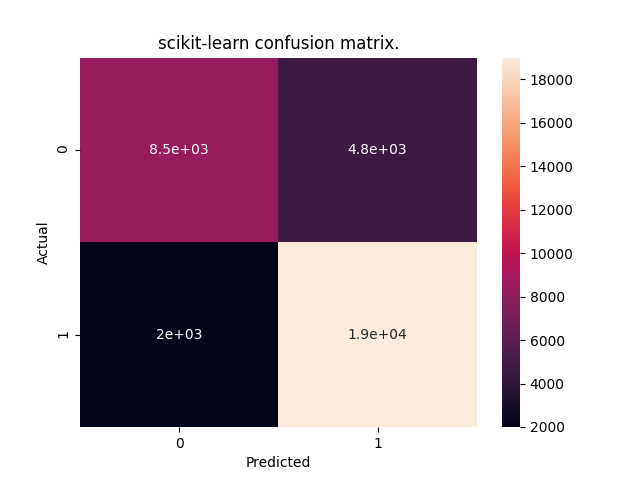
\includegraphics[scale=0.6]{images/confusion_skl.png}
    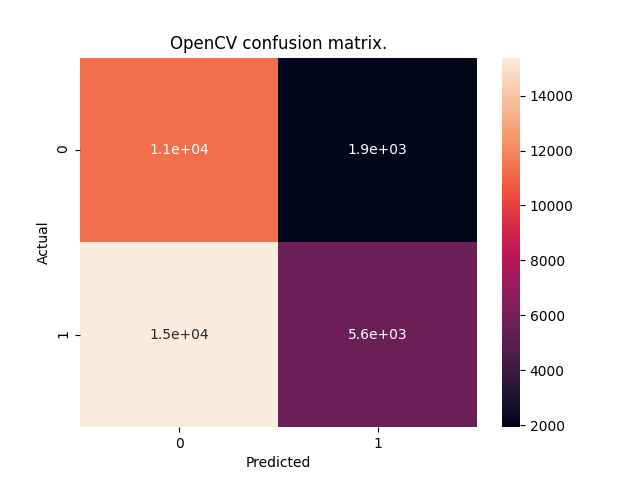
\includegraphics[scale=0.6]{images/confusion_cv2.png}
    \caption{Confusion matrices.}
    \label{fig:confusion}
\end{figure}

\begin{table}[h!t]
    \centering
    \caption{Scores for the classifiers.}
    \label{tab:scores}
    \begin{tabular}{lcc}
        & scikit-learn & OpenCV \\
        Accuracy & 0.805 & 0.491 \\
        Precision & 0.814 & 0.421 \\
        Recall & 0.639 & 0.860 \\
        F1 & 0.358 & 0.283 \\
    \end{tabular}
\end{table}

They're not particularly good, except maybe accuracy and precision, but is clear how scikit-learn's classifier is more balanced. 
Even in recall, where OpenCV performs better, the difference is less significant than the cases in which scikit-learn is better.

In image \ref{fig:roc} the ROC curves for the scikit-learn SVM classifier and OpenCV ones are plotted.
For OpenCV where considered three different classifiers: a linear one, a polynomial one with degree 3 and, for comparision, an RBF one.

The polynomial one has terrible performances, is like throwing chances \footnote{With an AUC of 0.5}, while the linear and RBF ones overlap each other with quite better performances.
Again the best performing classifier is the scikit-learn with a RBF kernel, the AUCs are displayed in table \ref{tab:auc}.

\begin{table}[h!t]
    \centering
    \caption{Scores for the classifiers.}
    \label{tab:auc}
    \begin{tabular}{lcc}
        & scikit & OpenCV \\
        AUC & 0.774 & 0.560 \\
    \end{tabular}
\end{table}

Also the DET curves for the scikit-learn and OpenCV, both with the RBF kernel, were plot in figure \ref{fig:det} and again the scikit-learn model is better than the OpenCV one.

On figure \ref{fig:eet} are plotted the false positive (i.e. false genuine) error rate and the false negative (i.e. false rejection) one, the intersection point is the equal error rate (EER) and the ideal threshold seems to be 1.25.
Keep in mind that these two error rates are plotted against only three thresholds so this value does not necessarly match the best threshold. 
The EET is identified only for the scikit-learn SVM since it is the best model so far.

\begin{figure}[h!t]
    \centering
    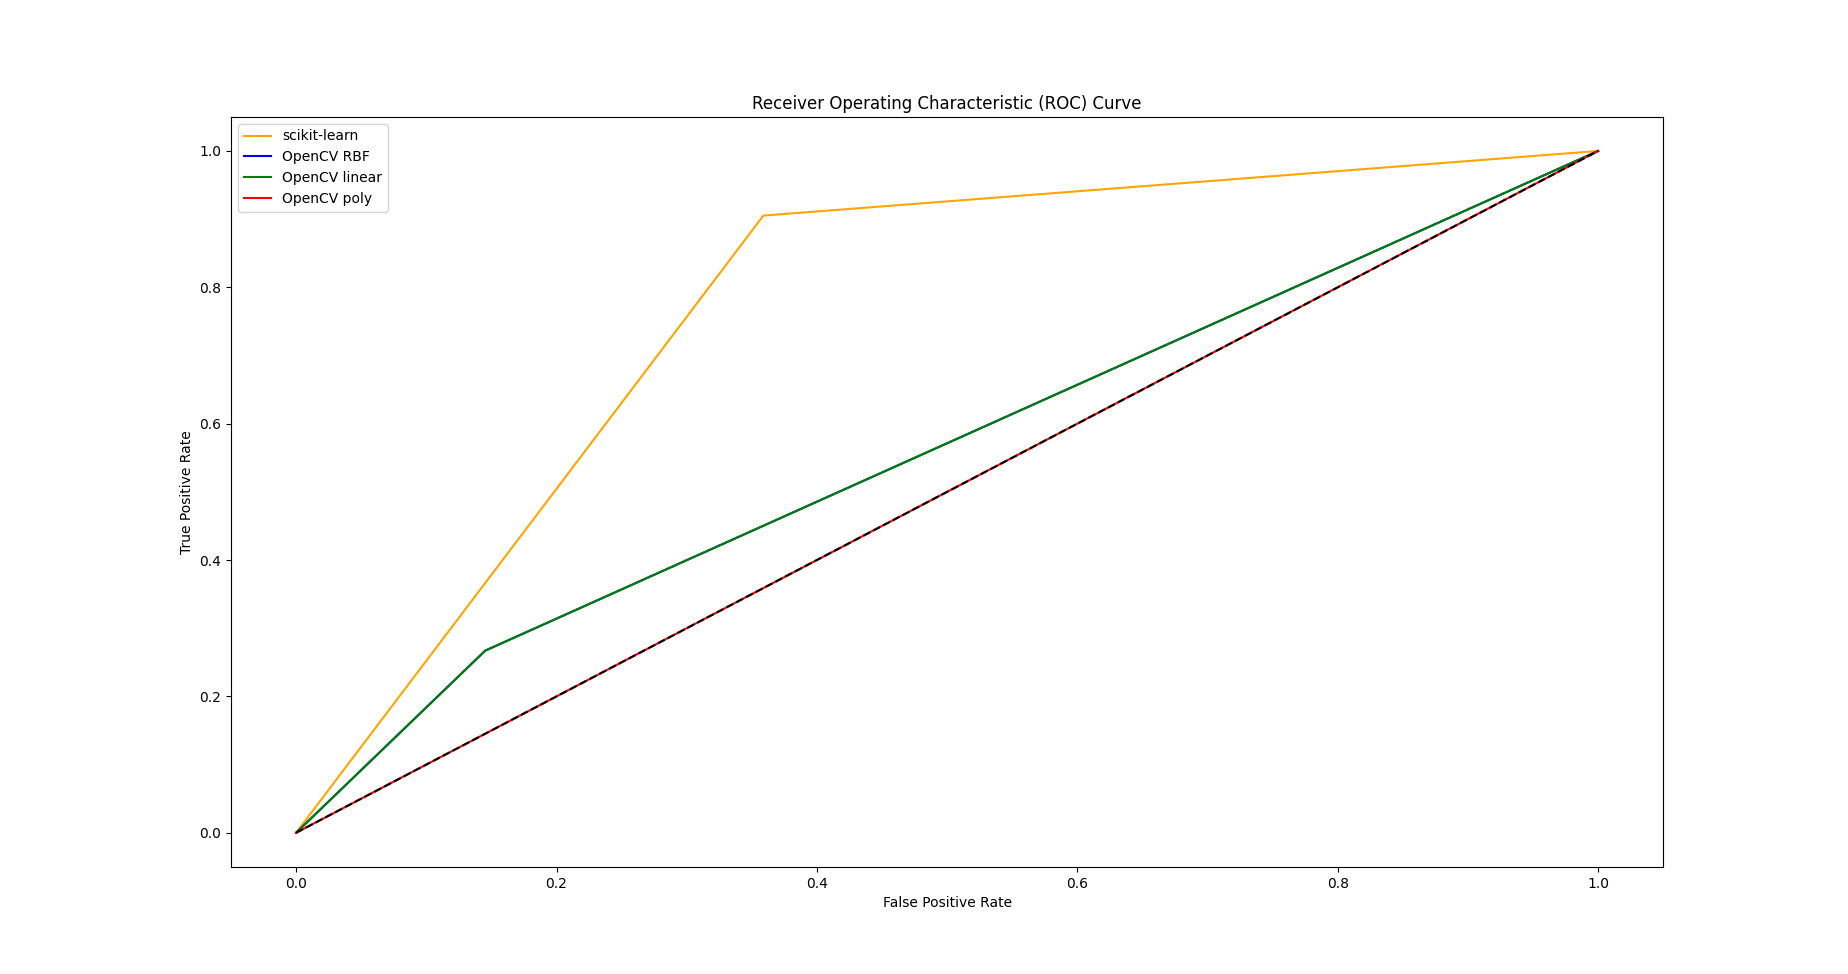
\includegraphics[scale=0.25]{images/roc.png}
    \caption{ROC.}
    \label{fig:roc}
\end{figure}

\begin{figure}[h!t]
    \centering
    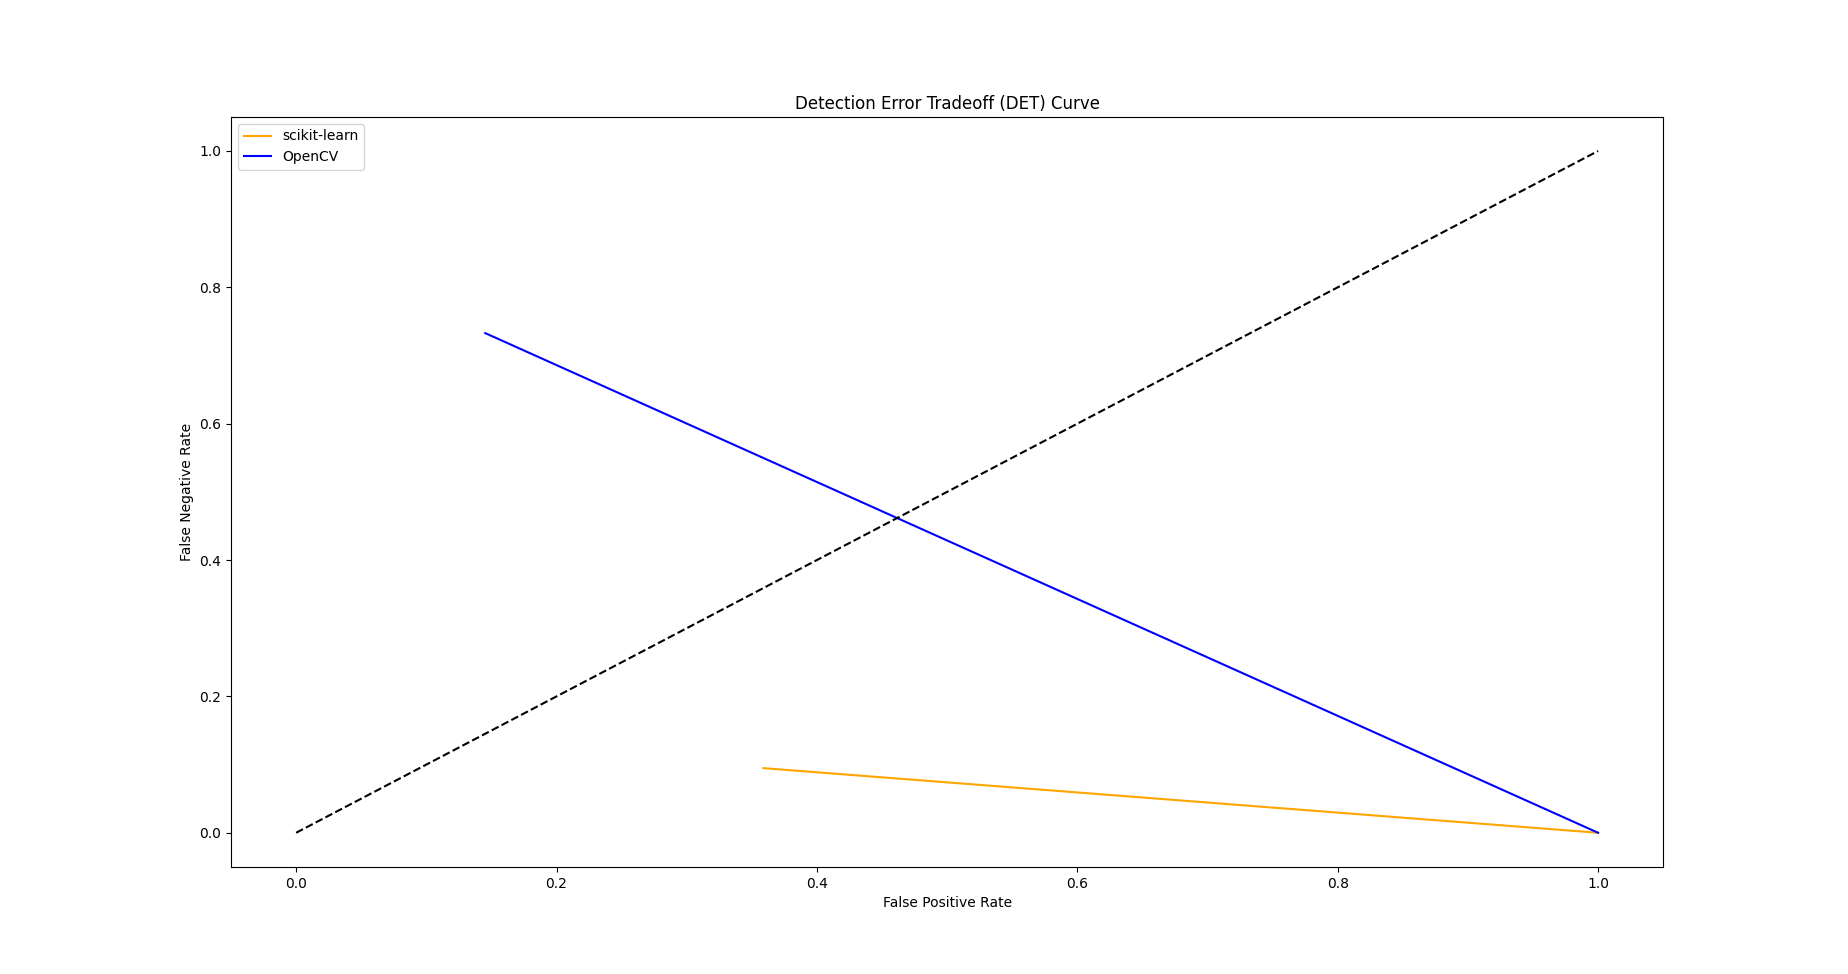
\includegraphics[scale=0.25]{images/det.png}
    \caption{DET.}
    \label{fig:det}
\end{figure}

\begin{figure}[h!t]
    \centering
    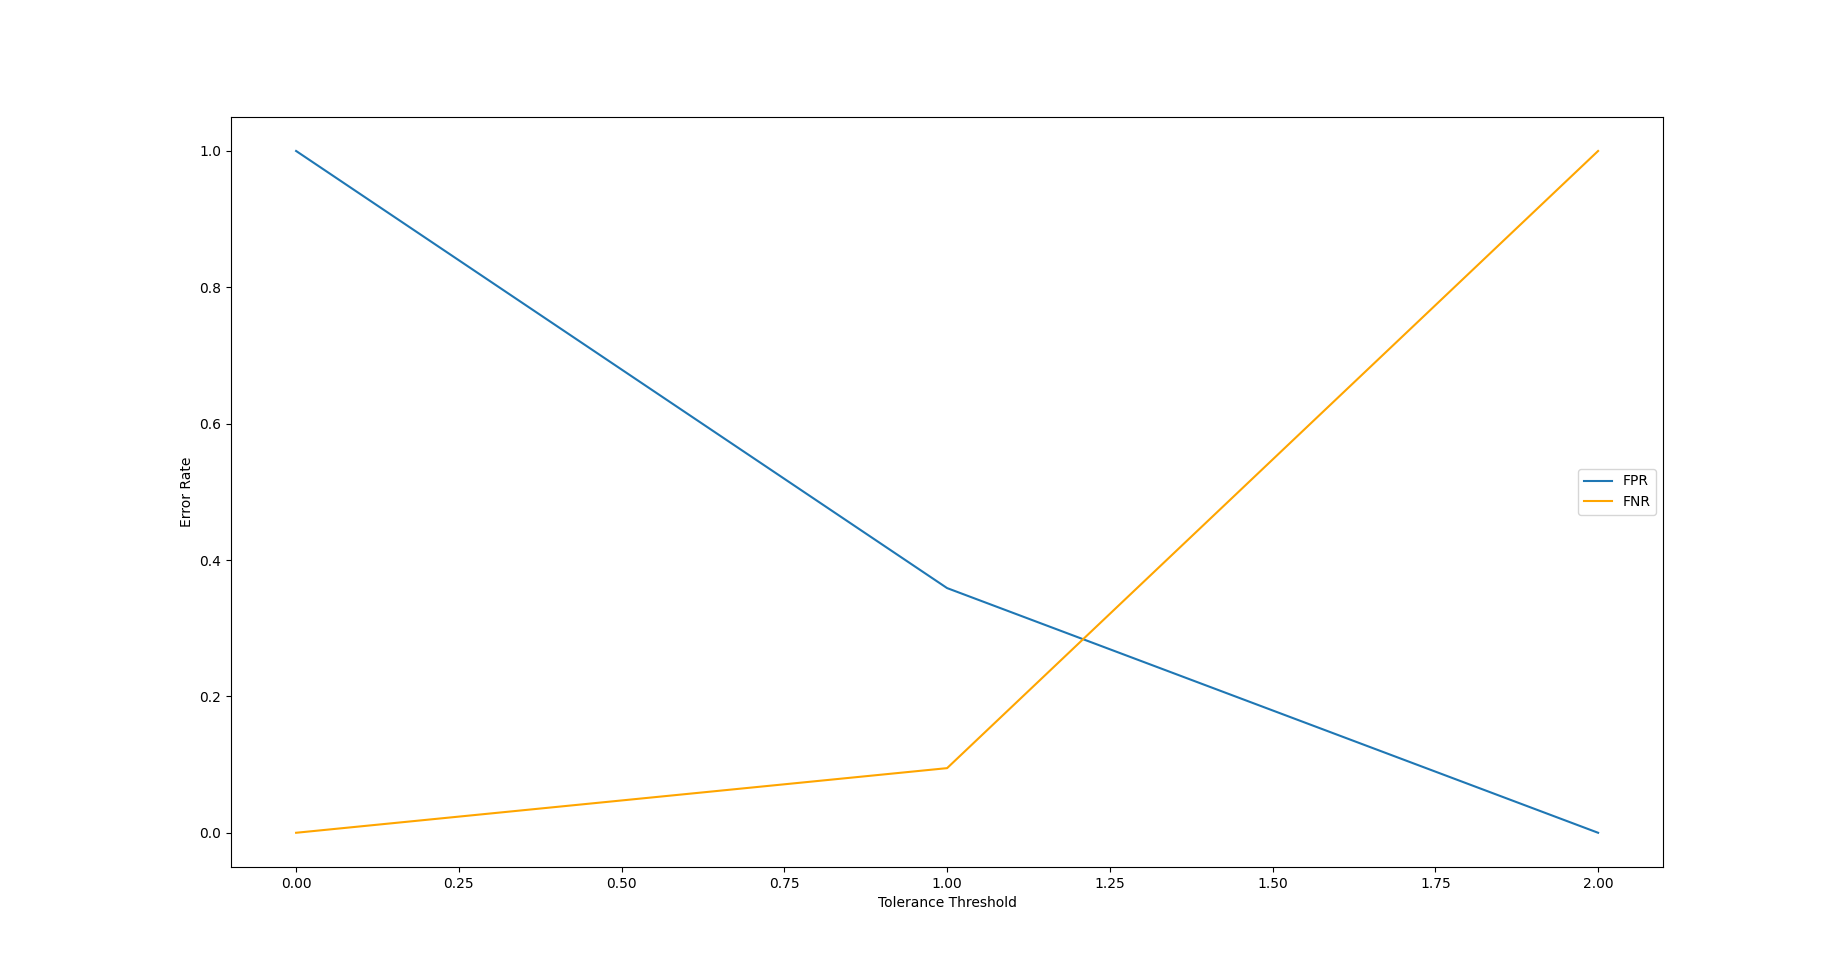
\includegraphics[scale=0.25]{images/eet.png}
    \caption{EET.}
    \label{fig:eet}
\end{figure}
